\begin{frame}{WebRTC Protocols}
\begin{tikzpicture}
\node at (0,0) {\includegraphics[page=18,width=\textwidth]{image/webrtc.pdf}};
%\node[align=center, nounibaredII, font=\footnotesize] at (3.5,-3.5) {In some cases, hole punching\\ fails, and a TURN Media Relay\\ on the public Internet must be used.};
%\node[align=center, nounibaredII] at (-3,-3) {Traversal of UDP\\ aRound NAT, RFC 5766};
\end{tikzpicture}
\end{frame}

\begin{frame}{A Joint Standards Effort}
\begin{itemize}
\item World Wide Web Consortium (W3C)
\begin{itemize}
\item Standardizing APIs
\item Most work in WEBRTC Working Group
\item Used by JavaScript to access RTC function
\end{itemize}
\item Internet Engineering Task Force (IETF)
\begin{itemize}
\item Standardizing protocols (bit on wire)
\item Codecs 
\item Peer Connection will use RTP, SDP, and extensions
\item Some work in RTCWEB Working Group
\item Lots of related work in MMUSIC, AVTCORE, etc.
\end{itemize}
\end{itemize}
\end{frame}

\begin{frame}{OPUS Audio Codec}\framesubtitle{Comparison}
\begin{tikzpicture}
\node at (0,0) {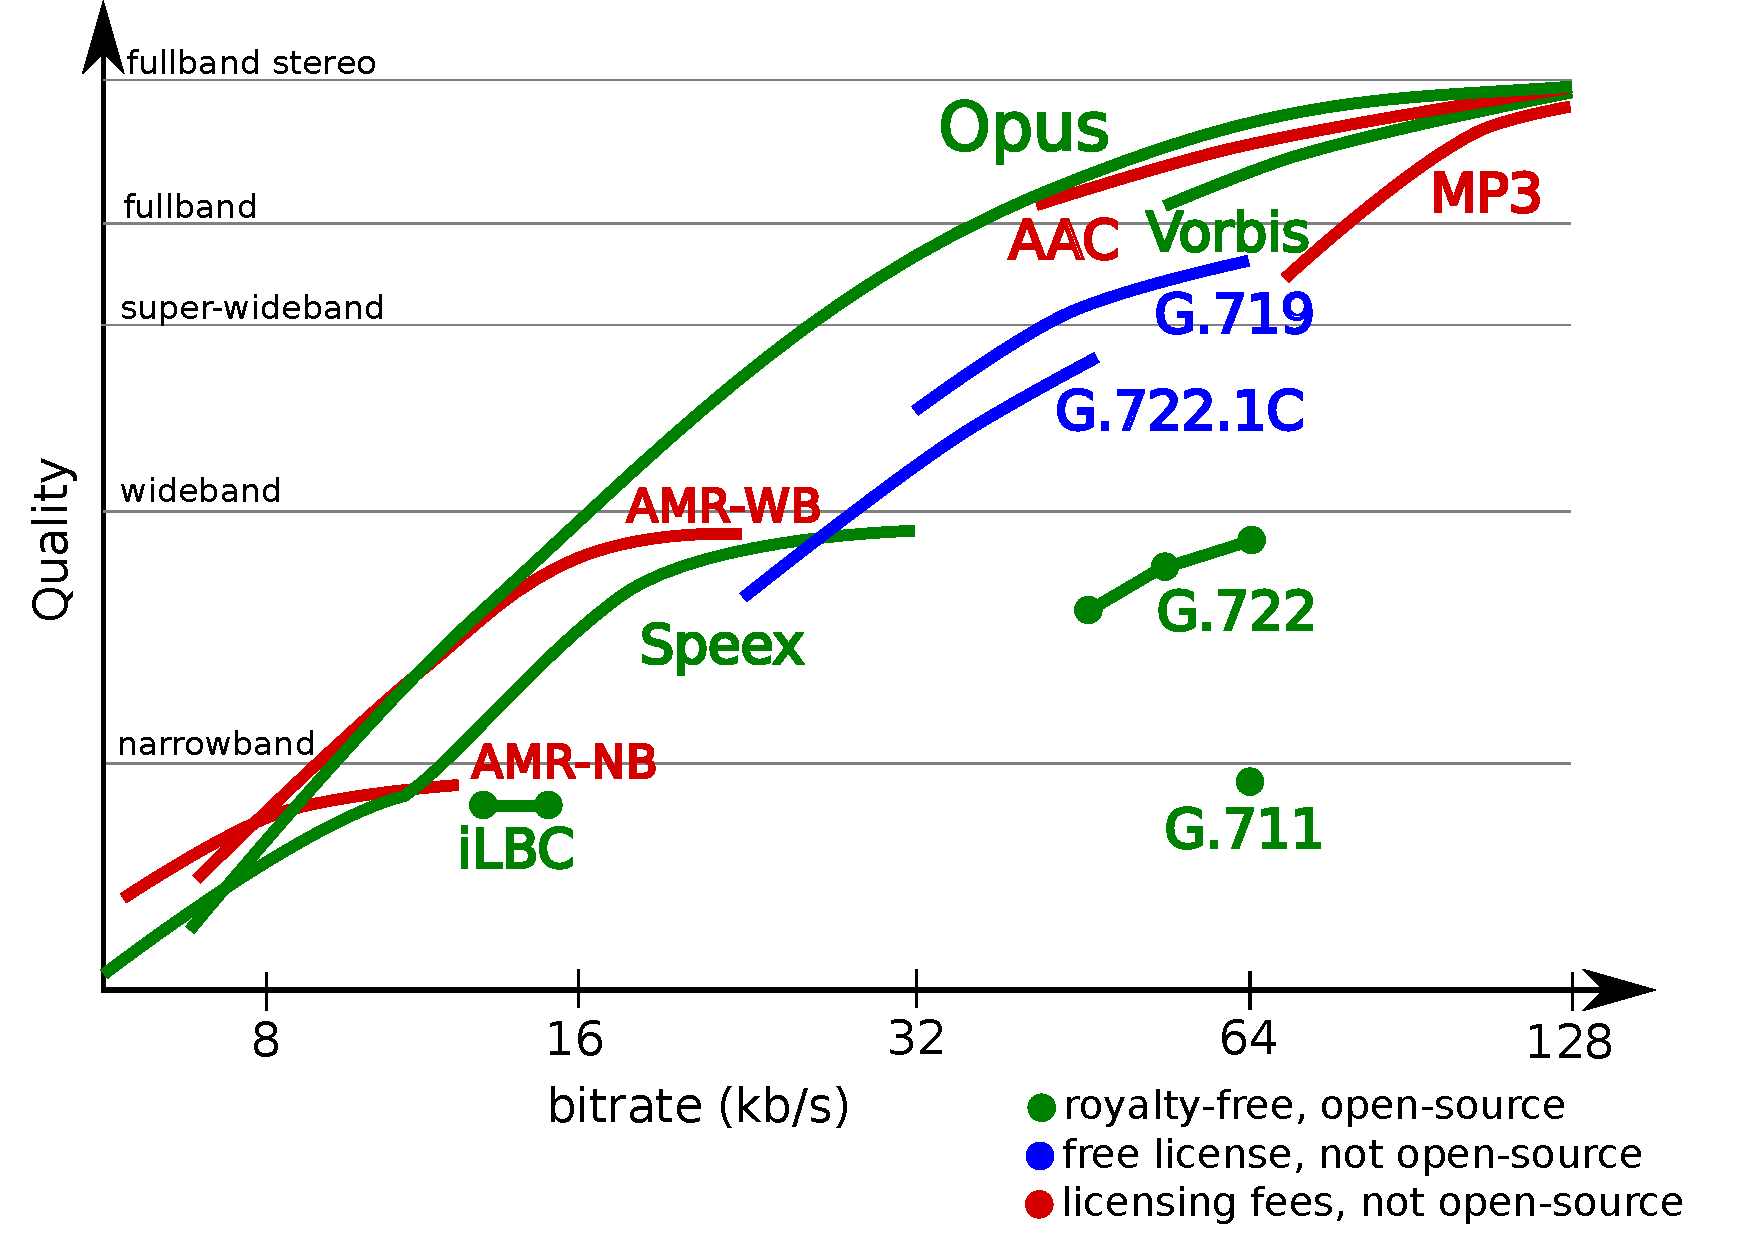
\includegraphics[height=.9\textheight]{image/opus.pdf}};
%\node[align=center, nounibaredII, font=\footnotesize] at (3.5,-3.5) {In some cases, hole punching\\ fails, and a TURN Media Relay\\ on the public Internet must be used.};
%\node[align=center, nounibaredII] at (-3,-3) {Traversal of UDP\\ aRound NAT, RFC 5766};
\end{tikzpicture}
\end{frame}

\begin{frame}{Standard Codecs in WebRTC}
\begin{small}
\begin{longtable}{|c|p{.5\textwidth}|c|}
\hline
Codec & Use & Specification\\
\hline
%\endhead
\hline
Opus & Narrowband to wideband Internet audio codec for speech and music & RFC 6716\\
\hline
G.711 & PCM audio encoding for PSTN interworking and backwards compatibility with VoIP systems & RFC 3551\\
\hline
Telephone Events & Transport of Dual Tone Multi Frequency (DTMF) tones & RFC 4733\\
\hline
H.264 & Video codec requiring licensing & RFC 6184\\
\hline
VP8 & Open source video codec & RFC 6386\\
\hline
\end{longtable}
\end{small}
\begin{itemize}
\item Mandatory to Implement (MTI) audio codecs settled on Opus and G.711 (finally!)
\item Video is not yet settled (H.264 vs. VP8 fight!)
\end{itemize}
\end{frame}

\begin{frame}{WebRTC and the Enterprise}
\begin{itemize}
\item Enterprise has unique requirements on WebRTC
\item Security
\begin{itemize}
\item Firewall traversal
\item Access control
\item Peer-to-peer data flows
\end{itemize}
\item Compliance
\begin{itemize}
\item Recording \& logging
\item Policy compliance
\end{itemize}
\item Integration with existing infrastructure
\item New element proposed
\begin{itemize}
\item ``Secure Edge'' located in enterprise DMZ
\end{itemize}
\end{itemize}
\end{frame}

\begin{frame}{What's Next?}
\begin{itemize}
\item W3C and IETF standards still need to be finalized
\item Browsers need to add support
\begin{itemize}
\item Chrome and Firefox browser have much of this functionality now!
\item Their mobile derivatives are almost on the same level. 
\end{itemize}
\item Mandatory to Implement video codec needs to be decided
\item Enterprise use of WebRTC need to be worked out
\end{itemize}
\end{frame}